\documentclass[compress,red]{beamer}
\usepackage[utf8]{inputenc}
\usepackage{ucs}
\usepackage{amsmath}
\usepackage{amsfonts}
\usepackage{amssymb}
\usepackage[russian]{babel}
\usepackage{graphicx}
\usepackage{wrapfig}

\usepackage{tikz}
\usepackage{verbatim}

\usepackage{color}
\usepackage{xcolor}
\usepackage{listings}

\usepackage{caption}

\lstset{
language=ruby,
extendedchars=\true,
inputencoding=utf8x,
commentstyle=\itshape,
stringstyle=\bf,
belowcaptionskip=5pt }


\DeclareCaptionFont{white}{\color{white}}
\DeclareCaptionFormat{listing}{\colorbox{gray}{\parbox{\textwidth}{#1#2#3}}}
\captionsetup[lstlisting]{format=listing,labelfont=white,textfont=white}

\usetikzlibrary{calc,trees,positioning,arrows,chains,shapes.geometric,%
    decorations.pathreplacing,decorations.pathmorphing,shapes,%
    matrix,shapes.symbols}

\tikzset{
>=stealth',
  punktchain/.style={
    rectangle, 
    rounded corners, 
    % fill=black!10,
    draw=black, very thick,
    text width=10em, 
    minimum height=3em, 
    text centered, 
    on chain},
  line/.style={draw, thick, <-},
  element/.style={
    tape,
    top color=white,
    bottom color=blue!50!black!60!,
    minimum width=8em,
    draw=blue!40!black!90, very thick,
    text width=10em, 
    minimum height=1.5em, 
    text centered, 
    on chain},
  every join/.style={->, thick,shorten <=1pt},
  decoration={brace},
  tuborg/.style={decorate},
  tubnode/.style={midway, right=2pt},
}

\mode<presentation>

\usetheme{Warsaw}

\definecolor{Red}{rgb}{1,0,0}
\definecolor{Blue}{rgb}{0,0,1}
\definecolor{Green}{rgb}{0,1,0}
\definecolor{magenta}{rgb}{1,0,.6}
\definecolor{lightblue}{rgb}{0,.5,1}
\definecolor{lightpurple}{rgb}{.6,.4,1}
\definecolor{gold}{rgb}{.6,.5,0}
\definecolor{orange}{rgb}{1,0.4,0}
\definecolor{hotpink}{rgb}{1,0,0.5}
\definecolor{newcolor2}{rgb}{.5,.3,.5}
\definecolor{newcolor}{rgb}{0,.3,1}
\definecolor{newcolor3}{rgb}{1,0,.35}
\definecolor{darkgreen1}{rgb}{0, .35, 0}
\definecolor{darkgreen}{rgb}{0, .6, 0}
\definecolor{darkred}{rgb}{.75,0,0}

\xdefinecolor{olive}{cmyk}{0.64,0,0.95,0.4}
\xdefinecolor{purpleish}{cmyk}{0.75,0.75,0,0}

\useoutertheme[subsection=false]{smoothbars}

\title{Разбор итоговых задач}
\author{Информатика \\ 10-11 классы}

%\usecolortheme{dolphin}


\begin{document}
%%титульная страница
\maketitle
%% основные моменты

\section{Задачи}

\subsection{Массивы}
\begin{frame}[fragile]
  \frametitle{Задача 1}
  \begin{itemize}
    \item Дан целочисленный массив из 30 элементов. Элементы могут принимать значения от 0 до 100 – баллы, полученные на ЕГЭ. Опишите на русском языке или на одном из языков программирования алгоритм, который подсчитывает и выводит средний балл учащихся, сдавших экзамен (получивших оценку более 20 баллов). Гарантируется, что хотя бы один ученик в классе успешно сдал экзамен.
  \end{itemize}
\end{frame}

\subsection{Пример}
\begin{frame}[fragile]
  \frametitle{Пример}
  \centerline{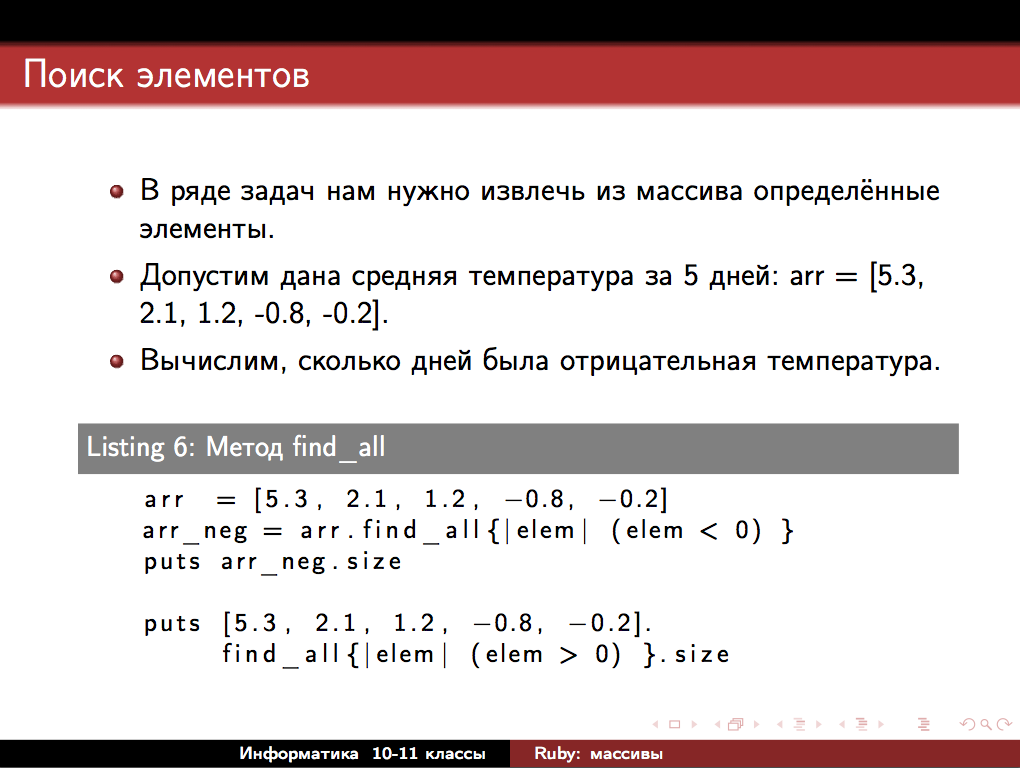
\includegraphics[width=0.8\textwidth]{images/screen1.png}}
\end{frame}

\subsection{Два}
\begin{frame}[fragile]
  \frametitle{Работа со строками}
  \begin{itemize}
    \item Напишите программу, подсчитывающую максимальное количество подряд идущих отрицательных элементов в целочисленном массиве длины 30.
    \item Напишите программу, подсчитывающую максимальное количество подряд идущих элементов массива, каждый из которых больше предыдущего. Длина массива — 30 элементов.
    \item На вход программы подается содержится текст на английском языке, заканчивающийся точкой (другие символы “.” в тексте отсутствуют). Требуется написать программу, которая будет определять и выводить на экран английскую букву, встречающуюся в этом тексте чаще всего, и количество там таких букв. Строчные и прописные буквы при этом считаются не различимыми. Если искомых букв несколько, то программа должна выводить на экран первую из них по алфавиту. Например, пусть файл содержит следующую запись: \textbf{It is not a simple task. Yes!} 
Чаще всего здесь встречаются буквы I, S и T (слово Yes в подсчете не учитывается, так как расположено после точки). Следовательно, в данном случае программа должна вывести два символа, разделенных пробелом: I 3
  \end{itemize}
\end{frame}

\subsection{Три}
\begin{frame}[fragile]
  \frametitle{Динамическое программирование}
  \begin{itemize}
    \item На вход программе подаются сведения о телефонах всех сотрудников некоторого учреждения. В первой строке сообщается количество сотрудников N, каждая из следующих N строк имеет следующий формат: 
    \item Фамилия Инициалы телефон
    \item где Фамилия --- строка, состоящая не более чем из 20 символов, Инициалы --- строка, состоящая не более чем из 4-х символов (буква, точка, буква, точка), <телефон> --- семизначный номер, 3-я и 4, я, а также 5-я и 6-я цифры которого разделены символом ---. Фамилия и Инициалы, а также Инициалы и телефон разделены одним пробелом.
    \item Пример входной строки: Иванов П.С. 555-66-77
  \end{itemize}
\end{frame}

\subsection{Три-2}
\begin{frame}[fragile]
  \frametitle{Динамическое программирование}
  \begin{itemize}
    \item Сотрудники одного подразделения имеют один и тот же номер телефона. Номера телефонов в учреждении отличаются только двумя последними цифрами. Требуется написать как можно более эффективную программу, которая будет выводить на экран информацию, сколько в среднем сотрудников работает в одном подразделении данного учреждения.
  \end{itemize}
\end{frame}

\subsection{Четыре}
\begin{frame}[fragile]
  \frametitle{Диофантовы уравнения}
  \begin{itemize}
    \item Напишите эффективную программу, находящую все решения линейного диофантова уравнения $ax+by=c$,
    \item где $a, b, c$ --- натуральные числа, задающиеся в начале программы, $x, y$ --- неизвестные (\textbf{целые числа}).
    \item Ограничение: $x,y < 100$; то есть надо найти решения, где оба неизвестных не превосходят $100$.
  \end{itemize}
\end{frame}

\section{References}
\subsection{References}
\begin{frame}[fragile]
  \frametitle{References}
  \begin{itemize}
    \item При подготовке данного материала использовались сайты: http://ru.wikibooks.org/wiki/Ruby, http://rubydev.ru, http://en.wikipedia.org, http://ruby-lang.org.
    \item Все презентации доступны на http://school.smirik.ru!
    \item Вопросы, предложения, д/з: smirik@gmail.com
  \end{itemize}
\end{frame}

\end{document}